% fig_mem_stage.tex - mem_stage (rtl/mem_stage.sv): load/store unit (store side
% and load side of one lsu instance) around the data memory.
\documentclass[tikz,border=8pt]{standalone}
\usepackage[T1]{fontenc}
\usepackage{lmodern}
\usepackage[scaled=0.92]{helvet}
\renewcommand{\familydefault}{\sfdefault}
% rv32i_style.tex - shared TikZ styles for the single-cycle RV32I diagrams.
% Visual language (same as the course PDF):
%   thick border, blue fill  = holds state (clocked)
%   thin border, white fill  = combinational logic
%   green trapezium          = multiplexer (0/1 marks the input chosen by select)
%   dashed orange            = control signal;  solid navy = data
%   /32 on a wire            = bus width;       dot = wires joined
% Port names are the exact SystemVerilog port names of the module drawn.
\usetikzlibrary{arrows.meta, positioning, calc, fit, backgrounds, shapes.geometric, shapes.misc}

\definecolor{ink}{RGB}{31,56,100}
\definecolor{statefill}{RGB}{220,230,242}
\definecolor{muxdraw}{RGB}{56,118,59}
\definecolor{muxfill}{RGB}{226,239,218}
\definecolor{ctrl}{RGB}{197,90,17}
\definecolor{ctrlfill}{RGB}{252,232,216}
\definecolor{note}{RGB}{110,110,110}
\definecolor{tintIF}{RGB}{236,243,251}
\definecolor{tintID}{RGB}{240,247,235}
\definecolor{tintEX}{RGB}{255,246,229}
\definecolor{tintMEM}{RGB}{244,237,249}
\definecolor{tintWB}{RGB}{233,246,245}

\tikzset{
  >={Stealth[length=2.2mm,width=1.6mm]},
  wire/.style      = {draw=ink, line width=0.75pt},
  data/.style      = {wire, ->},
  ctl/.style       = {draw=ctrl, line width=0.75pt, dashed, dash pattern=on 3pt off 1.6pt, ->},
  ctlnoarrow/.style= {draw=ctrl, line width=0.75pt, dashed, dash pattern=on 3pt off 1.6pt},
  block/.style     = {draw=ink, line width=0.75pt, fill=white, rectangle, align=center,
                      inner sep=3pt, font=\small},
  state/.style     = {block, line width=1.8pt, fill=statefill},
  ctrlblock/.style = {block, draw=ctrl, fill=ctrlfill},
  muxst/.style     = {draw=muxdraw, fill=muxfill, line width=0.9pt},
  aluSt/.style     = {draw=ink, fill=white, line width=0.9pt},
  addr/.style      = {circle, draw=ink, fill=white, line width=0.75pt, inner sep=0.5pt,
                      minimum size=6.5mm, font=\large},
  stage/.style     = {draw=ink!70, rounded corners=6pt, line width=0.9pt},
  sig/.style       = {font=\scriptsize\ttfamily, text=ink, inner sep=1.2pt},
  csig/.style      = {font=\scriptsize\ttfamily, text=ctrl, inner sep=1.2pt},
  wlbl/.style      = {font=\tiny, text=ink, inner sep=0.8pt},
  notetxt/.style   = {font=\scriptsize\itshape, text=note, align=left},
  mlbl/.style      = {font=\tiny\bfseries, text=muxdraw, inner sep=0pt},
  title/.style     = {font=\large\bfseries, text=ink},
  dot/.style       = {circle, fill=ink, inner sep=0pt, minimum size=4pt},
  cdot/.style      = {circle, fill=ctrl, inner sep=0pt, minimum size=4pt},
  portbox/.style   = {rectangle, fill=ink, inner sep=0pt, minimum size=4pt},
  cportbox/.style  = {rectangle, fill=ctrl, inner sep=0pt, minimum size=4pt},
  flag/.style      = {sig, draw=ink, fill=white, rounded corners=1.5pt, inner sep=1.5pt},  % net label
  stub/.style      = {ctl},                                                                 % named select input
}

% Two-line block label: module name, then "instance : module".
\newcommand{\blk}[2]{\textbf{#1}\\[-1pt]{\scriptsize\ttfamily #2}}
% Same with a two-line name.
\newcommand{\blkII}[3]{\textbf{#1}\\[-2pt]\textbf{#2}\\[-1pt]{\scriptsize\ttfamily #3}}

% Bus-width mark on a horizontal wire: \wmark{(x,y)}{32}
\newcommand{\wmark}[2]{%
  \draw[draw=ink, line width=0.6pt] ($#1+(-0.07,-0.13)$) -- ($#1+(0.07,0.13)$);
  \node[wlbl, above] at ($#1+(0,0.1)$) {#2};}
% Bus-width mark on a vertical wire: \wmarkv{(x,y)}{32}
\newcommand{\wmarkv}[2]{%
  \draw[draw=ink, line width=0.6pt] ($#1+(-0.13,-0.07)$) -- ($#1+(0.13,0.07)$);
  \node[wlbl, right] at ($#1+(0.1,0)$) {#2};}

% Multiplexer, inputs on the left, output on the right.
% \muxR{name}{x}{y}{height}: defines (name-out), (name-top), (name-bot), (name-l) (left x).
\newcommand{\muxR}[4]{%
  \draw[muxst] ($(#2,#3)+(-0.28,-#4/2)$) -- ($(#2,#3)+(-0.28,#4/2)$)
               -- ($(#2,#3)+(0.28,#4/2-0.28)$) -- ($(#2,#3)+(0.28,-#4/2+0.28)$) -- cycle;
  \coordinate (#1-out) at ($(#2,#3)+(0.28,0)$);
  \coordinate (#1-top) at ($(#2,#3)+(0,#4/2-0.14)$);
  \coordinate (#1-bot) at ($(#2,#3)+(0,-#4/2+0.14)$);
  \coordinate (#1-l)   at ($(#2,#3)+(-0.28,0)$);}

% ALU shape (notched trapezium), inputs a (upper) and b (lower) on the left.
% \aluR{name}{x}{y}{height}: defines (name-a), (name-b), (name-out), (name-op) (top edge).
\newcommand{\aluR}[4]{%
  \draw[aluSt] ($(#2,#3)+(-0.65,#4/2)$) -- ($(#2,#3)+(0.65,#4/4)$) -- ($(#2,#3)+(0.65,-#4/4)$)
               -- ($(#2,#3)+(-0.65,-#4/2)$) -- ($(#2,#3)+(-0.65,-0.28)$) -- ($(#2,#3)+(-0.35,0)$)
               -- ($(#2,#3)+(-0.65,0.28)$) -- cycle;
  \coordinate (#1-a)   at ($(#2,#3)+(-0.65,#4*0.3)$);
  \coordinate (#1-b)   at ($(#2,#3)+(-0.65,-#4*0.3)$);
  \coordinate (#1-out) at ($(#2,#3)+(0.65,0)$);
  \coordinate (#1-op)  at ($(#2,#3)+(0,#4*0.375)$);
  \coordinate (#1-c)   at ($(#2,#3)+(0.12,0)$);}

% Ports on a stage boundary. \inport{x}{y}{name}{width}  (label to the left)
% The width may be empty (1-bit port); it is expanded first so \foreach variables work.
\newcommand{\portw}[1]{\edef\pwtmp{#1}\ifx\pwtmp\empty\else\,[\pwtmp]\fi}
\newcommand{\inport}[4]{%
  \node[portbox] at (#1,#2) {};
  \node[sig, anchor=east] at ($(#1,#2)+(-0.12,0)$) {#3\portw{#4}};}
\newcommand{\cinport}[4]{%
  \node[cportbox] at (#1,#2) {};
  \node[csig, anchor=east] at ($(#1,#2)+(-0.12,0)$) {#3\portw{#4}};}
\newcommand{\outport}[4]{%
  \node[portbox] at (#1,#2) {};
  \node[sig, anchor=west] at ($(#1,#2)+(0.12,0)$) {#3\portw{#4}};}
\newcommand{\coutport}[4]{%
  \node[cportbox] at (#1,#2) {};
  \node[csig, anchor=west] at ($(#1,#2)+(0.12,0)$) {#3\portw{#4}};}
% Control input port on the top edge (label above).
\newcommand{\ctopport}[4]{%
  \node[cportbox] at (#1,#2) {};
  \node[csig, anchor=south] at ($(#1,#2)+(0,0.1)$) {#3\portw{#4}};}
% Data input port on the top edge (label above).
\newcommand{\topport}[4]{%
  \node[portbox] at (#1,#2) {};
  \node[sig, anchor=south] at ($(#1,#2)+(0,0.1)$) {#3\portw{#4}};}

% Legend strip. \legend{x}{y}
\newcommand{\legend}[2]{%
  \begin{scope}[shift={(#1,#2)}, font=\scriptsize]
    \node[state, minimum width=6mm, minimum height=3.5mm, inner sep=0pt] at (0,0) {};
    \node[anchor=west] at (0.45,0) {holds state};
    \node[block, minimum width=6mm, minimum height=3.5mm, inner sep=0pt] at (3.2,0) {};
    \node[anchor=west] at (3.65,0) {combinational};
    \draw[muxst] (6.2,-0.25) -- (6.2,0.25) -- (6.5,0.1) -- (6.5,-0.1) -- cycle;
    \node[anchor=west] at (6.6,0) {multiplexer};
    \draw[data] (8.7,0) -- (9.4,0); \node[anchor=west] at (9.45,0) {data};
    \draw[ctl] (10.4,0) -- (11.1,0); \node[anchor=west] at (11.15,0) {control};
    \node[portbox] at (12.6,0) {}; \node[anchor=west] at (12.7,0) {module port};
    \draw[wire] (14.6,0) -- (15.3,0); \draw[draw=ink, line width=0.6pt] (14.88,-0.13) -- (15.02,0.13);
    \node[wlbl] at (14.95,0.24) {32}; \node[anchor=west] at (15.35,0) {bus width};
  \end{scope}}

\begin{document}
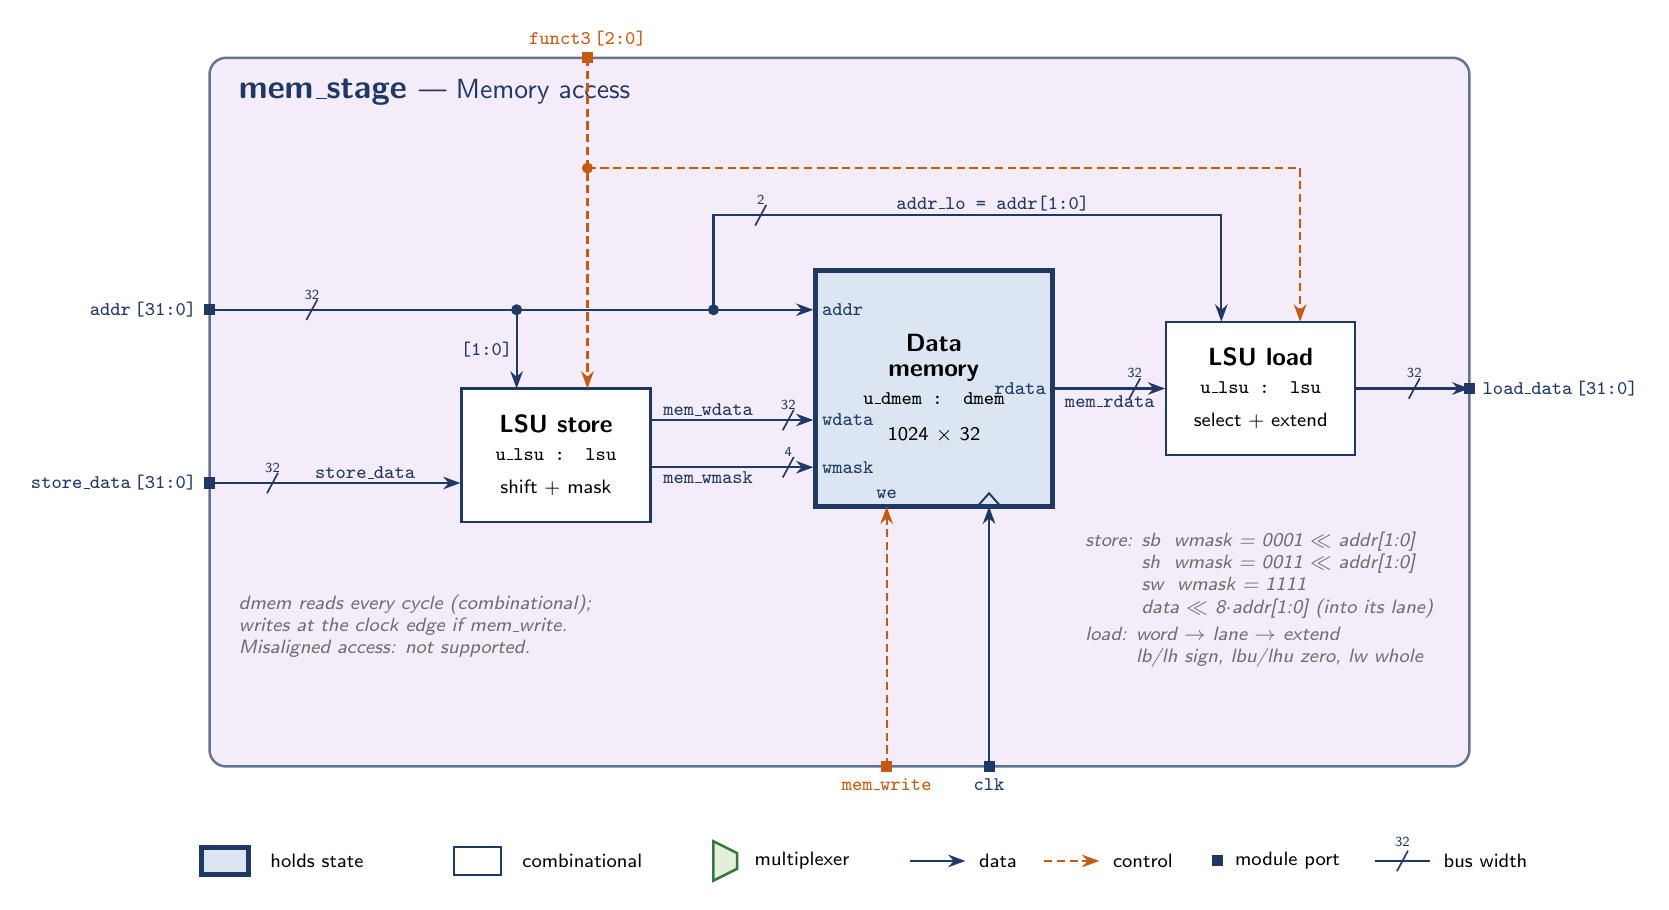
\begin{tikzpicture}
  % ---- stage boundary ----
  \draw[stage, fill=tintMEM] (0,0) rectangle (16,9);
  \node[title, anchor=north west] at (0.25,8.85) {mem\_stage \textmd{\normalsize --- Memory access}};

  % ---- ports ----
  \inport{0}{5.8}{addr}{31:0}
  \inport{0}{3.6}{store\_data}{31:0}
  \ctopport{4.8}{9}{funct3}{2:0}
  \node[cportbox] at (8.6,0) {};  \node[csig, anchor=north] at (8.6,-0.1) {mem\_write};
  \node[portbox]  at (9.9,0) {};  \node[sig,  anchor=north] at (9.9,-0.1) {clk};
  \outport{16}{4.8}{load\_data}{31:0}

  % ---- data memory ----
  \node[state, minimum width=30mm, minimum height=30mm] (dm) at (9.2,4.8)
        {\blkII{Data}{memory}{u\_dmem : dmem}\\[2pt]{\scriptsize 1024 $\times$ 32}};
  \node[sig, anchor=west] at (7.73,5.8) {addr};
  \node[sig, anchor=west] at (7.73,4.4) {wdata};
  \node[sig, anchor=west] at (7.73,3.8) {wmask};
  \node[sig, anchor=east] at (10.67,4.8) {rdata};
  \node[sig, anchor=south] at (8.6,3.35) {we};
  \draw[ink, line width=0.7pt] (9.75,3.3) -- (9.9,3.47) -- (10.05,3.3);   % clock-input mark

  % ---- LSU, store side ----
  \node[block, minimum width=24mm, minimum height=17mm] (ls) at (4.4,3.95)
        {\textbf{LSU store}\\[-1pt]{\scriptsize\ttfamily u\_lsu : lsu}\\[1pt]{\scriptsize shift + mask}};
  % ---- LSU, load side ----
  \node[block, minimum width=24mm, minimum height=17mm] (ll) at (13.35,4.8)
        {\textbf{LSU load}\\[-1pt]{\scriptsize\ttfamily u\_lsu : lsu}\\[1pt]{\scriptsize select + extend}};

  % ---- wires ----
  \draw[data] (0,5.8) -- (dm.west |- 0,5.8);
  \draw[data] (0,3.6) -- node[sig, above, pos=0.62] {store\_data} (ls.west |- 0,3.6);
  \draw[data] (ls.east |- 0,4.4) -- node[sig, above, pos=0.35] {mem\_wdata} (dm.west |- 0,4.4);
  \draw[data] (ls.east |- 0,3.8) -- node[sig, below, pos=0.35] {mem\_wmask} (dm.west |- 0,3.8);
  \draw[data] (dm.east) -- node[sig, below=1pt] {mem\_rdata} (ll.west);
  \draw[data] (ll.east) -- (16,4.8);
  % addr[1:0] to both halves
  \node[dot] at (3.9,5.8) {};
  \draw[data] (3.9,5.8) -- node[sig, left, pos=0.5] {[1:0]} (3.9,4.8);
  \node[dot] at (6.4,5.8) {};
  \draw[data] (6.4,5.8) -- (6.4,7.0) -- node[sig, above, pos=0.55] {addr\_lo = addr[1:0]} (12.85,7.0) -- (12.85,5.65);
  % funct3 to both halves
  \node[cdot] at (4.8,7.6) {};
  \draw[ctl] (4.8,9) -- (4.8,4.8);
  \draw[ctl] (4.8,7.6) -- (13.85,7.6) -- (13.85,5.65);
  % memory write enable and clock from the bottom edge
  \draw[ctl]  (8.6,0) -- (8.6,3.3);
  \draw[data] (9.9,0) -- (9.9,3.3);

  % ---- bus widths ----
  \wmark{(1.3,5.8)}{32}
  \wmark{(0.8,3.6)}{32}
  \wmark{(7.35,4.4)}{32}
  \wmark{(7.35,3.8)}{4}
  \wmark{(11.75,4.8)}{32}
  \wmark{(15.3,4.8)}{32}
  \wmark{(7.0,7.0)}{2}

  % ---- notes ----
  \node[notetxt, anchor=north west] at (11.0,3.1)
       {store: sb\ \ wmask = 0001 $\ll$ addr[1:0]\\
        \hphantom{store: }sh\ \ wmask = 0011 $\ll$ addr[1:0]\\
        \hphantom{store: }sw\ \ wmask = 1111\\
        \hphantom{store: }data $\ll$ 8$\cdot$addr[1:0] (into its lane)\\[2pt]
        load: word $\rightarrow$ lane $\rightarrow$ extend\\
        \hphantom{load: }lb/lh sign, lbu/lhu zero, lw whole};
  \node[notetxt, anchor=north west] at (0.25,2.3)
       {dmem reads every cycle (combinational);\\writes at the clock edge if mem\_write.\\Misaligned access: not supported.};

  \legend{0.2}{-1.2}
\end{tikzpicture}
\end{document}
